\section{Detección de objetos con YOLO}
\label{sec:yolo-tecnologias}

La detección de objetos es una de las tareas principales dentro de la visión por computador. Su objetivo es localizar e identificar las instancias de una o varias clases presentes en una imagen, normalmente mediante cajas \textit{bounding box} asociadas a una etiqueta y a una puntuación de confianza. En esta sección se describe cómo YOLO afronta este problema.

\subsection{Modelo de detección YOLO}

Uno de los enfoques más utilizados para detección en tiempo real es YOLO \citep{RedmonYOLO2016}. Esta red neuronal convolucional plantea la detección como un problema de regresión directa sobre la imagen completa, prediciendo cajas y clases en una sola pasada. Esta filosofía de detector de una etapa resulta especialmente adecuada para vídeo, donde no basta con obtener buena precisión en imágenes aisladas, sino que también es importante mantener una velocidad de inferencia suficiente para procesar secuencias largas. Las implementaciones modernas de Ultralytics \citep{UltralyticsYOLO2023} \footnote{Ultralytics es una empresa y comunidad de desarrollo de software especializada en herramientas de visión por computador, conocida principalmente por mantener implementaciones modernas de YOLO y facilitar su entrenamiento, evaluación y despliegue.} han popularizado su uso práctico mediante modelos preentrenados, herramientas de entrenamiento y despliegue, y soporte para fine-tuning sobre datasets propios.


En la formulación original de YOLO, la imagen se divide en una cuadrícula de $S \times S$ celdas. Cada celda es responsable de predecir los objetos cuyo centro cae dentro de ella. Para cada celda, la red estima una o varias cajas delimitadoras junto con una confianza de objeto y una distribución de probabilidad sobre las clases. De forma simplificada, cada predicción puede representarse como:

\[
(x, y, w, h, C)
\]

donde $x$ e $y$ indican la posición del centro de la caja, $w$ y $h$ representan su anchura y altura, y $C$ expresa la confianza asociada a la existencia de un objeto y a la calidad de la localización. Además, la red predice las probabilidades de clase. La puntuación final de una detección puede entenderse como la combinación entre la confianza de objeto y la probabilidad de clase:

\[
score = P(\text{objeto}) \cdot P(\text{clase} \mid \text{objeto})
\]

El flujo de este modelo de detección se muestra en la \hyperref[fig:yolo-grid]{Figura~\ref*{fig:yolo-grid}}. La red comparte un mismo \textit{backbone} para extraer características visuales de la imagen y, a partir de ellas, produce simultáneamente la regresión de cajas, la confianza y la clasificación. Aunque las versiones modernas de YOLO utilizadas por implementaciones como Ultralytics han evolucionado respecto al modelo original, incorporando cabezas de detección multiescala y mejores funciones de pérdida, la idea central sigue siendo la misma: obtener cajas y clases directamente en una única pasada de la red.

\begin{figure}[H]
    \centering
    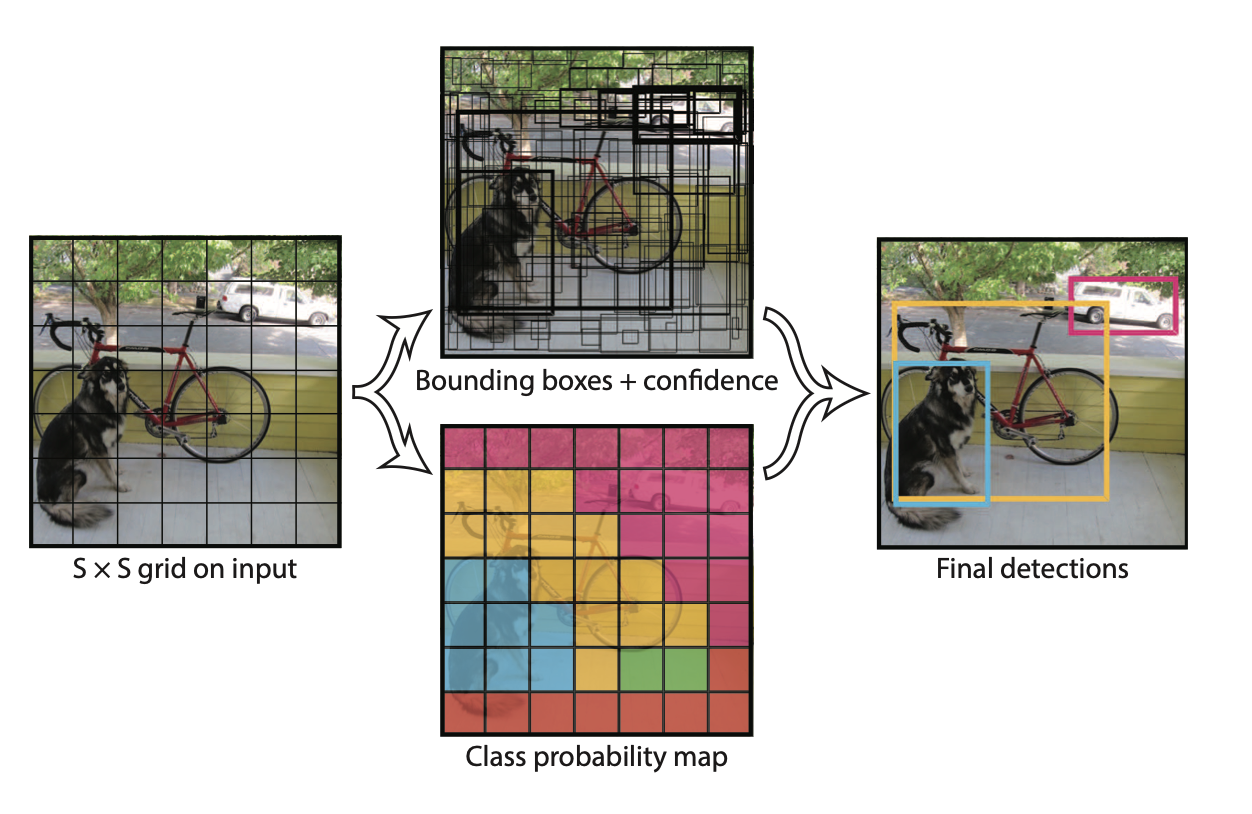
\includegraphics[width=0.9\textwidth]{Imagenes/Propias/YOLO2.png}
    \caption[Esquema conceptual de YOLO como detector de una etapa]{Esquema conceptual de YOLO como detector de una etapa: división espacial, regresión de cajas y clasificación. Fuente: reproducido de \citep{RedmonYOLO2016}.}
    \label{fig:yolo-grid}
\end{figure}

Durante el entrenamiento, la función de pérdida combina varios objetivos. Por un lado, penaliza el error de localización entre la caja predicha y la caja real. Por otro lado, penaliza los errores de confianza, diferenciando entre regiones que contienen objetos y regiones de fondo. Finalmente, incorpora el error de clasificación. Esto obliga al modelo a aprender simultáneamente tres tareas: localizar el objeto, decidir si realmente existe y asignarle una clase correcta.

\subsection{Post-procesado mediante Non-Maximum Suppression}
Tras la inferencia, es habitual que el detector produzca varias cajas muy próximas para un mismo objeto. Para eliminar estas detecciones redundantes se aplica \textit{Non-Maximum Suppression} (NMS). Este algoritmo ordena las cajas por puntuación, conserva la de mayor confianza y elimina aquellas cajas de la misma clase cuyo solape con ella supere un determinado umbral. El solape se mide mediante la intersección sobre la unión, o IoU:

\[
IoU(A,B)=\frac{\operatorname{area}(A \cap B)}{\operatorname{area}(A \cup B)}
\]

Si dos cajas tienen un IoU superior al umbral $\lambda_{nms}$, se considera que ambas representan el mismo objeto y se conserva únicamente la de mayor confianza. La \hyperref[fig:yolo-nms]{Figura~\ref*{fig:yolo-nms}} ilustra este proceso, en el que múltiples predicciones cercanas se reducen a una única caja final. Esto también puede observarse en el segundo paso de la \hyperref[fig:yolo-grid]{Figura~\ref*{fig:yolo-grid}}.

\begin{figure}[H]
    \centering
    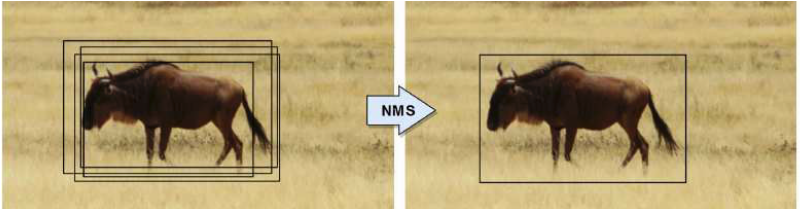
\includegraphics[width=0.9\textwidth]{Imagenes/Propias/YOLO1.png}
    \caption[Postproceso mediante Non-Maximum Suppression]{Postproceso mediante Non-Maximum Suppression para eliminar cajas redundantes.
    Fuente: reproducido de \citep{BesadaAnalisisSenal2025}}
    \label{fig:yolo-nms}
\end{figure}


\subsection{Métricas de evaluación en detección de objetos}
\label{subsec:metricas-deteccion-objetos}

Para evaluar un detector de objetos no basta con comprobar si predice la clase correcta, sino que también es necesario analizar la calidad de la localización espacial. Para ello se utiliza habitualmente la IoU. Una detección se considera correcta si su IoU supera un determinado umbral y la clase predicha coincide con la clase real.

A partir de esta correspondencia entre predicciones y anotaciones reales se calculan métricas como la precisión y el recall. La precisión mide qué proporción de las detecciones realizadas por el modelo son correctas, mientras que el recall mide qué proporción de los objetos reales han sido detectados. Estas métricas se definen como:

\[
\text{Precisión} = \frac{TP}{TP + FP}
\]

\[
\text{Recall} = \frac{TP}{TP + FN}
\]

donde $TP$ representa el número de verdaderos positivos, $FP$ el número de falsos positivos y $FN$ el número de falsos negativos. En el contexto de la detección de objetos, un verdadero positivo corresponde a una predicción cuya clase es correcta y cuya IoU con la caja real supera el umbral establecido. Un falso positivo es una detección incorrecta o duplicada, mientras que un falso negativo corresponde a un objeto real que no ha sido detectado.

El valor F1 combina ambas métricas mediante su media armónica:

\[
F1 = 2 \cdot \frac{\text{Precisión} \cdot \text{Recall}}{\text{Precisión} + \text{Recall}}
\]

Esta métrica resulta útil cuando se desea valorar conjuntamente falsos positivos, asociados a la precisión, y falsos negativos, asociados al recall.

En detección de objetos también es habitual emplear la métrica mAP (\textit{mean Average Precision}). El mAP@50 considera correcta una detección cuando alcanza un IoU mínimo de 0.50, mientras que el mAP@50-95 calcula el rendimiento medio usando varios umbrales de IoU entre 0.50 y 0.95.


\subsection{Papel de YOLO dentro del pipeline}
En este proyecto, YOLO se utiliza como detector inicial del pipeline para localizar jugadores, árbitros, porteros y balón en cada fotograma. Sus salidas sirven como entrada para las etapas posteriores de seguimiento y análisis temporal.

En esta sección se ha introducido YOLO desde un punto de vista conceptual. Su aplicación concreta dentro del sistema se desarrolla posteriormente en la \hyperref[sec:deteccion-elementos-juego]{Sección~\ref*{sec:deteccion-elementos-juego}, Detección de elementos del juego}.
